Jusqu'à présent, nous n'avons à aucun moment utiliser l'hyperbole $\setgeo{H}$ \squote{à deux branches} d'équation implicite $X^2 - 8 Y^2 = 1$ \textit{(on utilise ici des majuscules pour le système de coordonnées)}. C'est un peu dommage!%
\footnote{
    Cette section est née de l'échange avec Jérôme Germoni indiqué dans une précédente note de bas de page.
}


\medskip


Essayons de voir ce que donne le tracé de $M(x ; y)$ et $N(x' ; y')$ sur $\setgeo{H}$ autre que $E(1 ; 0)$, cf. le neutre de $\star$, et de $P(x'' ; y'')$
où
$\begin{pmatrix} 
  x'' \\ 
  y''
\end{pmatrix}
=
\begin{pmatrix}
  x \\ 
  y 
\end{pmatrix}
\star
\begin{pmatrix} 
  x' \\ 
  y'
\end{pmatrix}
=
\begin{pmatrix}
  x x' + 8 y y' \\ 
  x y' + x' y 
\end{pmatrix}$.
Nous avons que ce dernier point est aussi sur $\setgeo{H}$.


\medskip
%\newpage


\begin{multicols}{2}
	\center
	
	\fbox{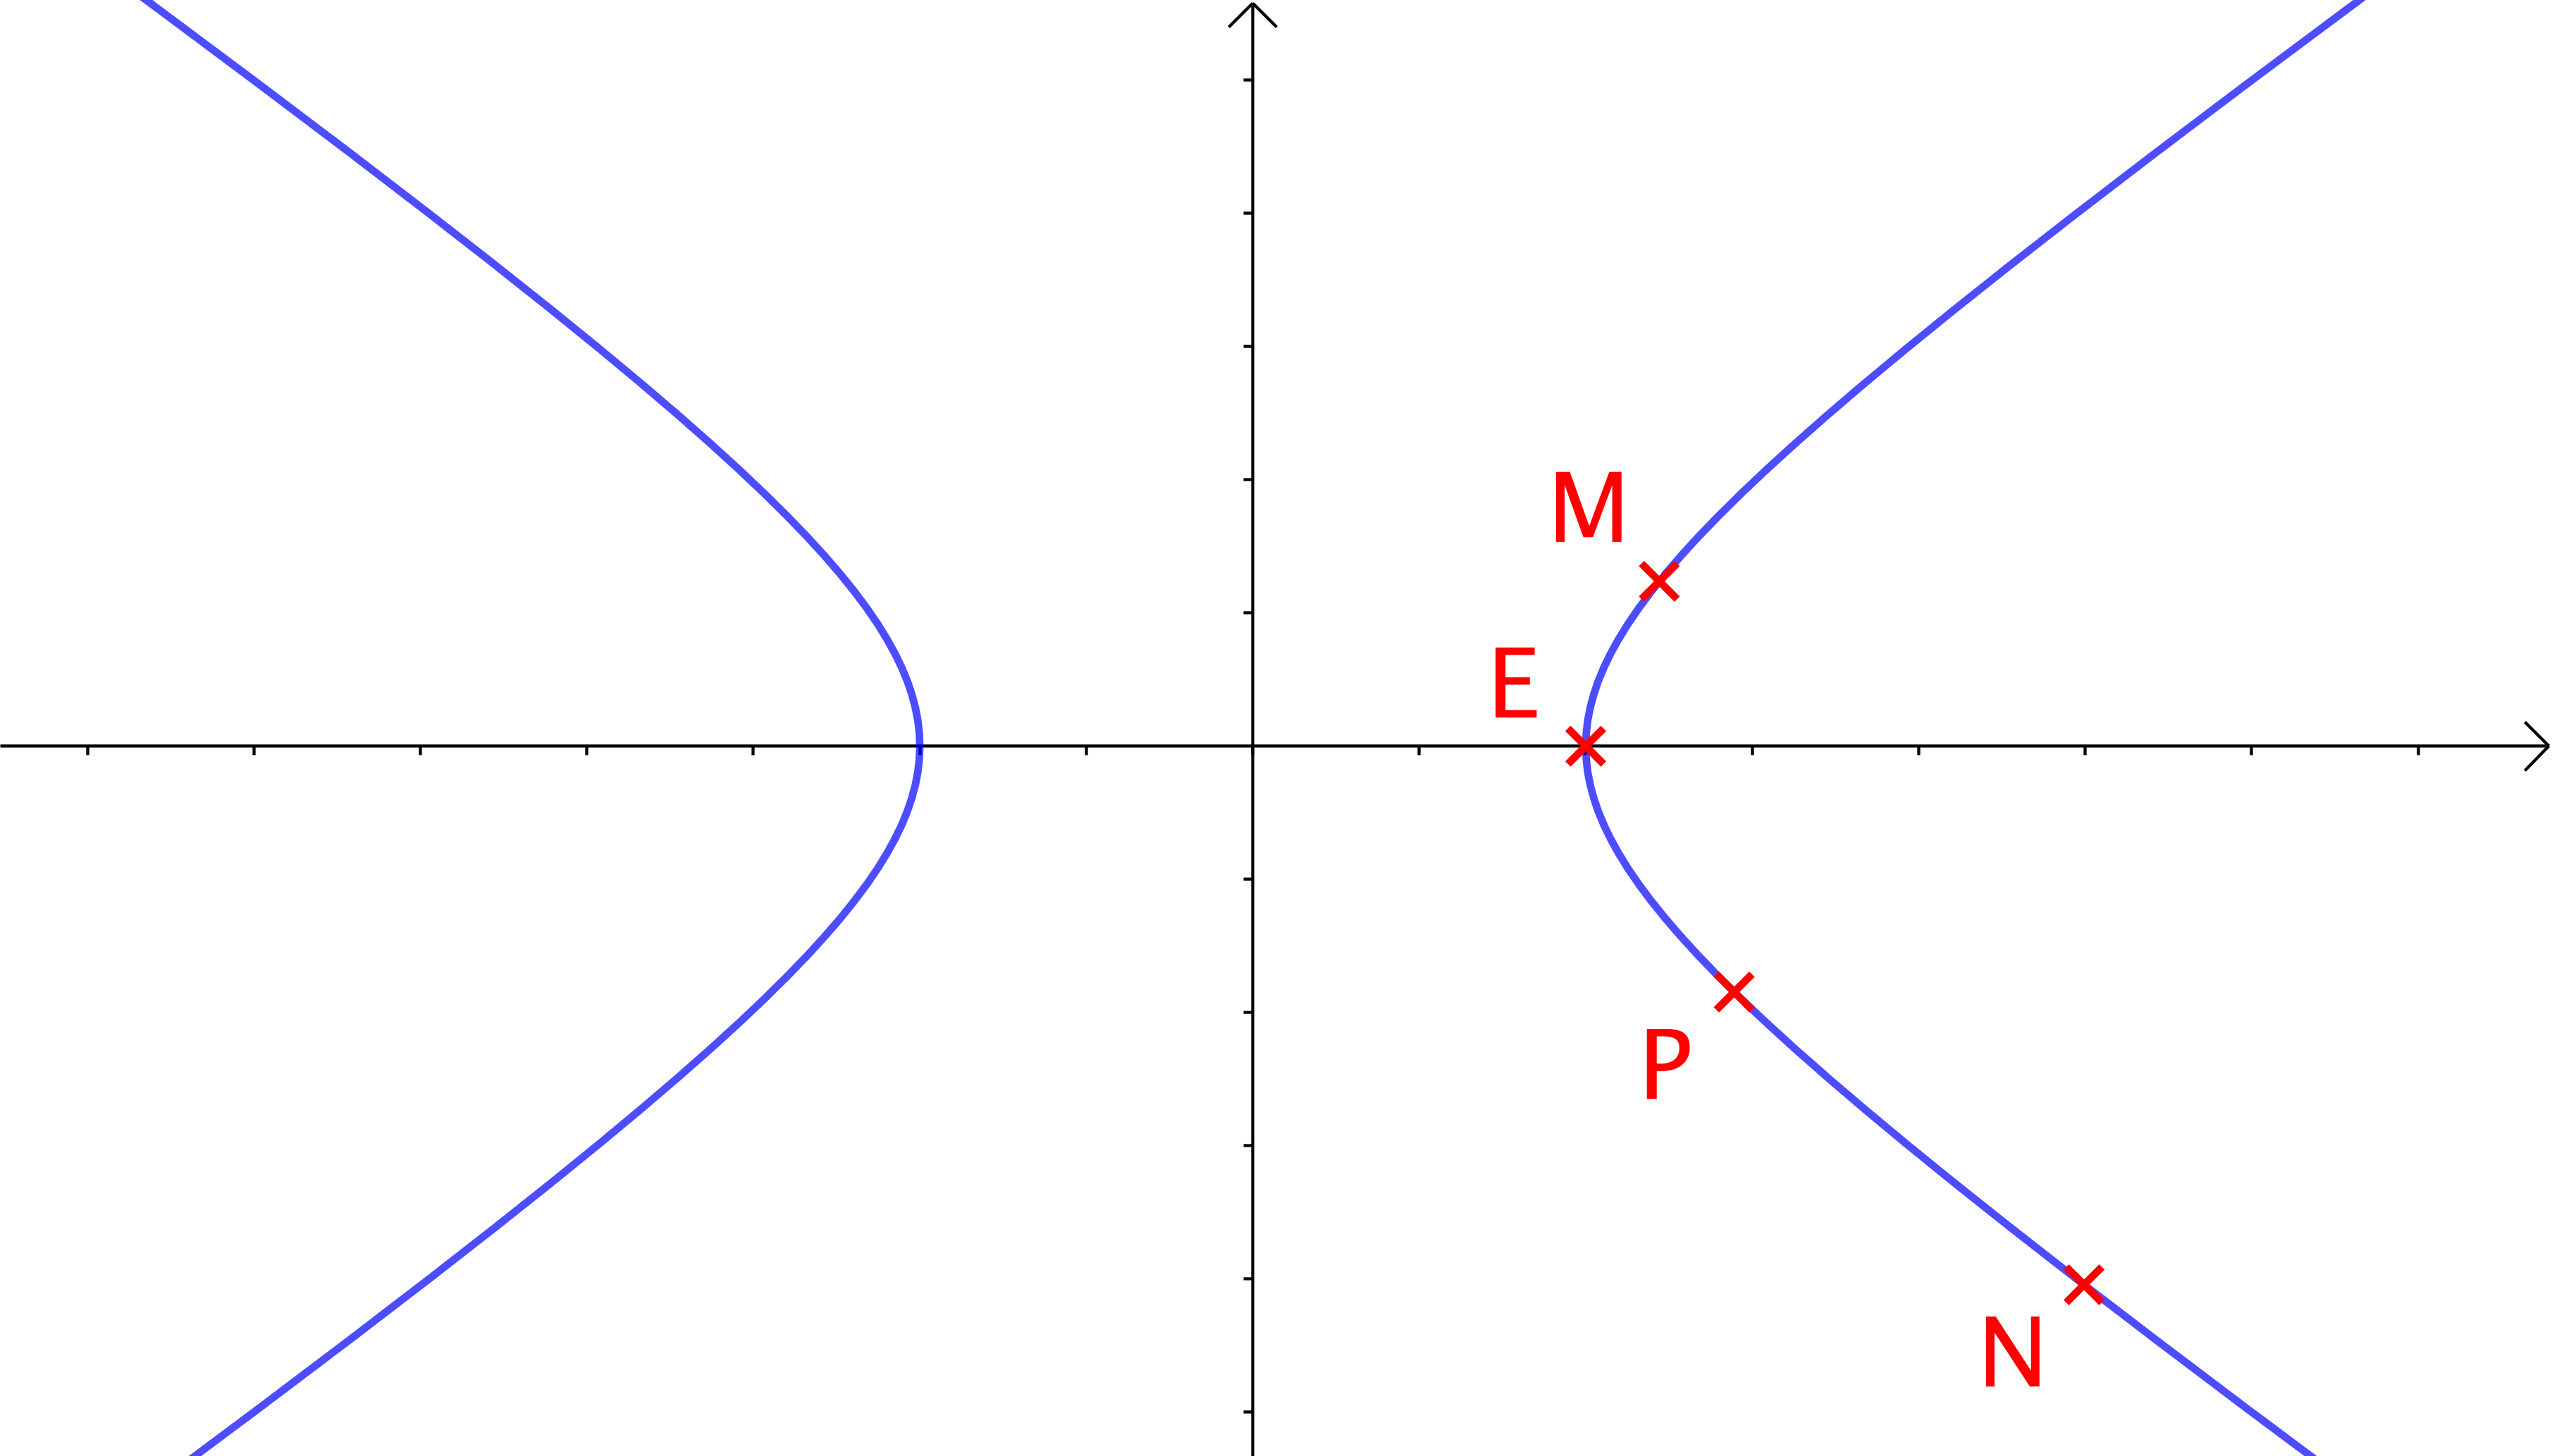
\includegraphics[scale =.5]{exo-spe-math-bac-s-juin-2018/geometry-is-the-queen/oblic-1.png}}
	
	\medskip
	
	\fbox{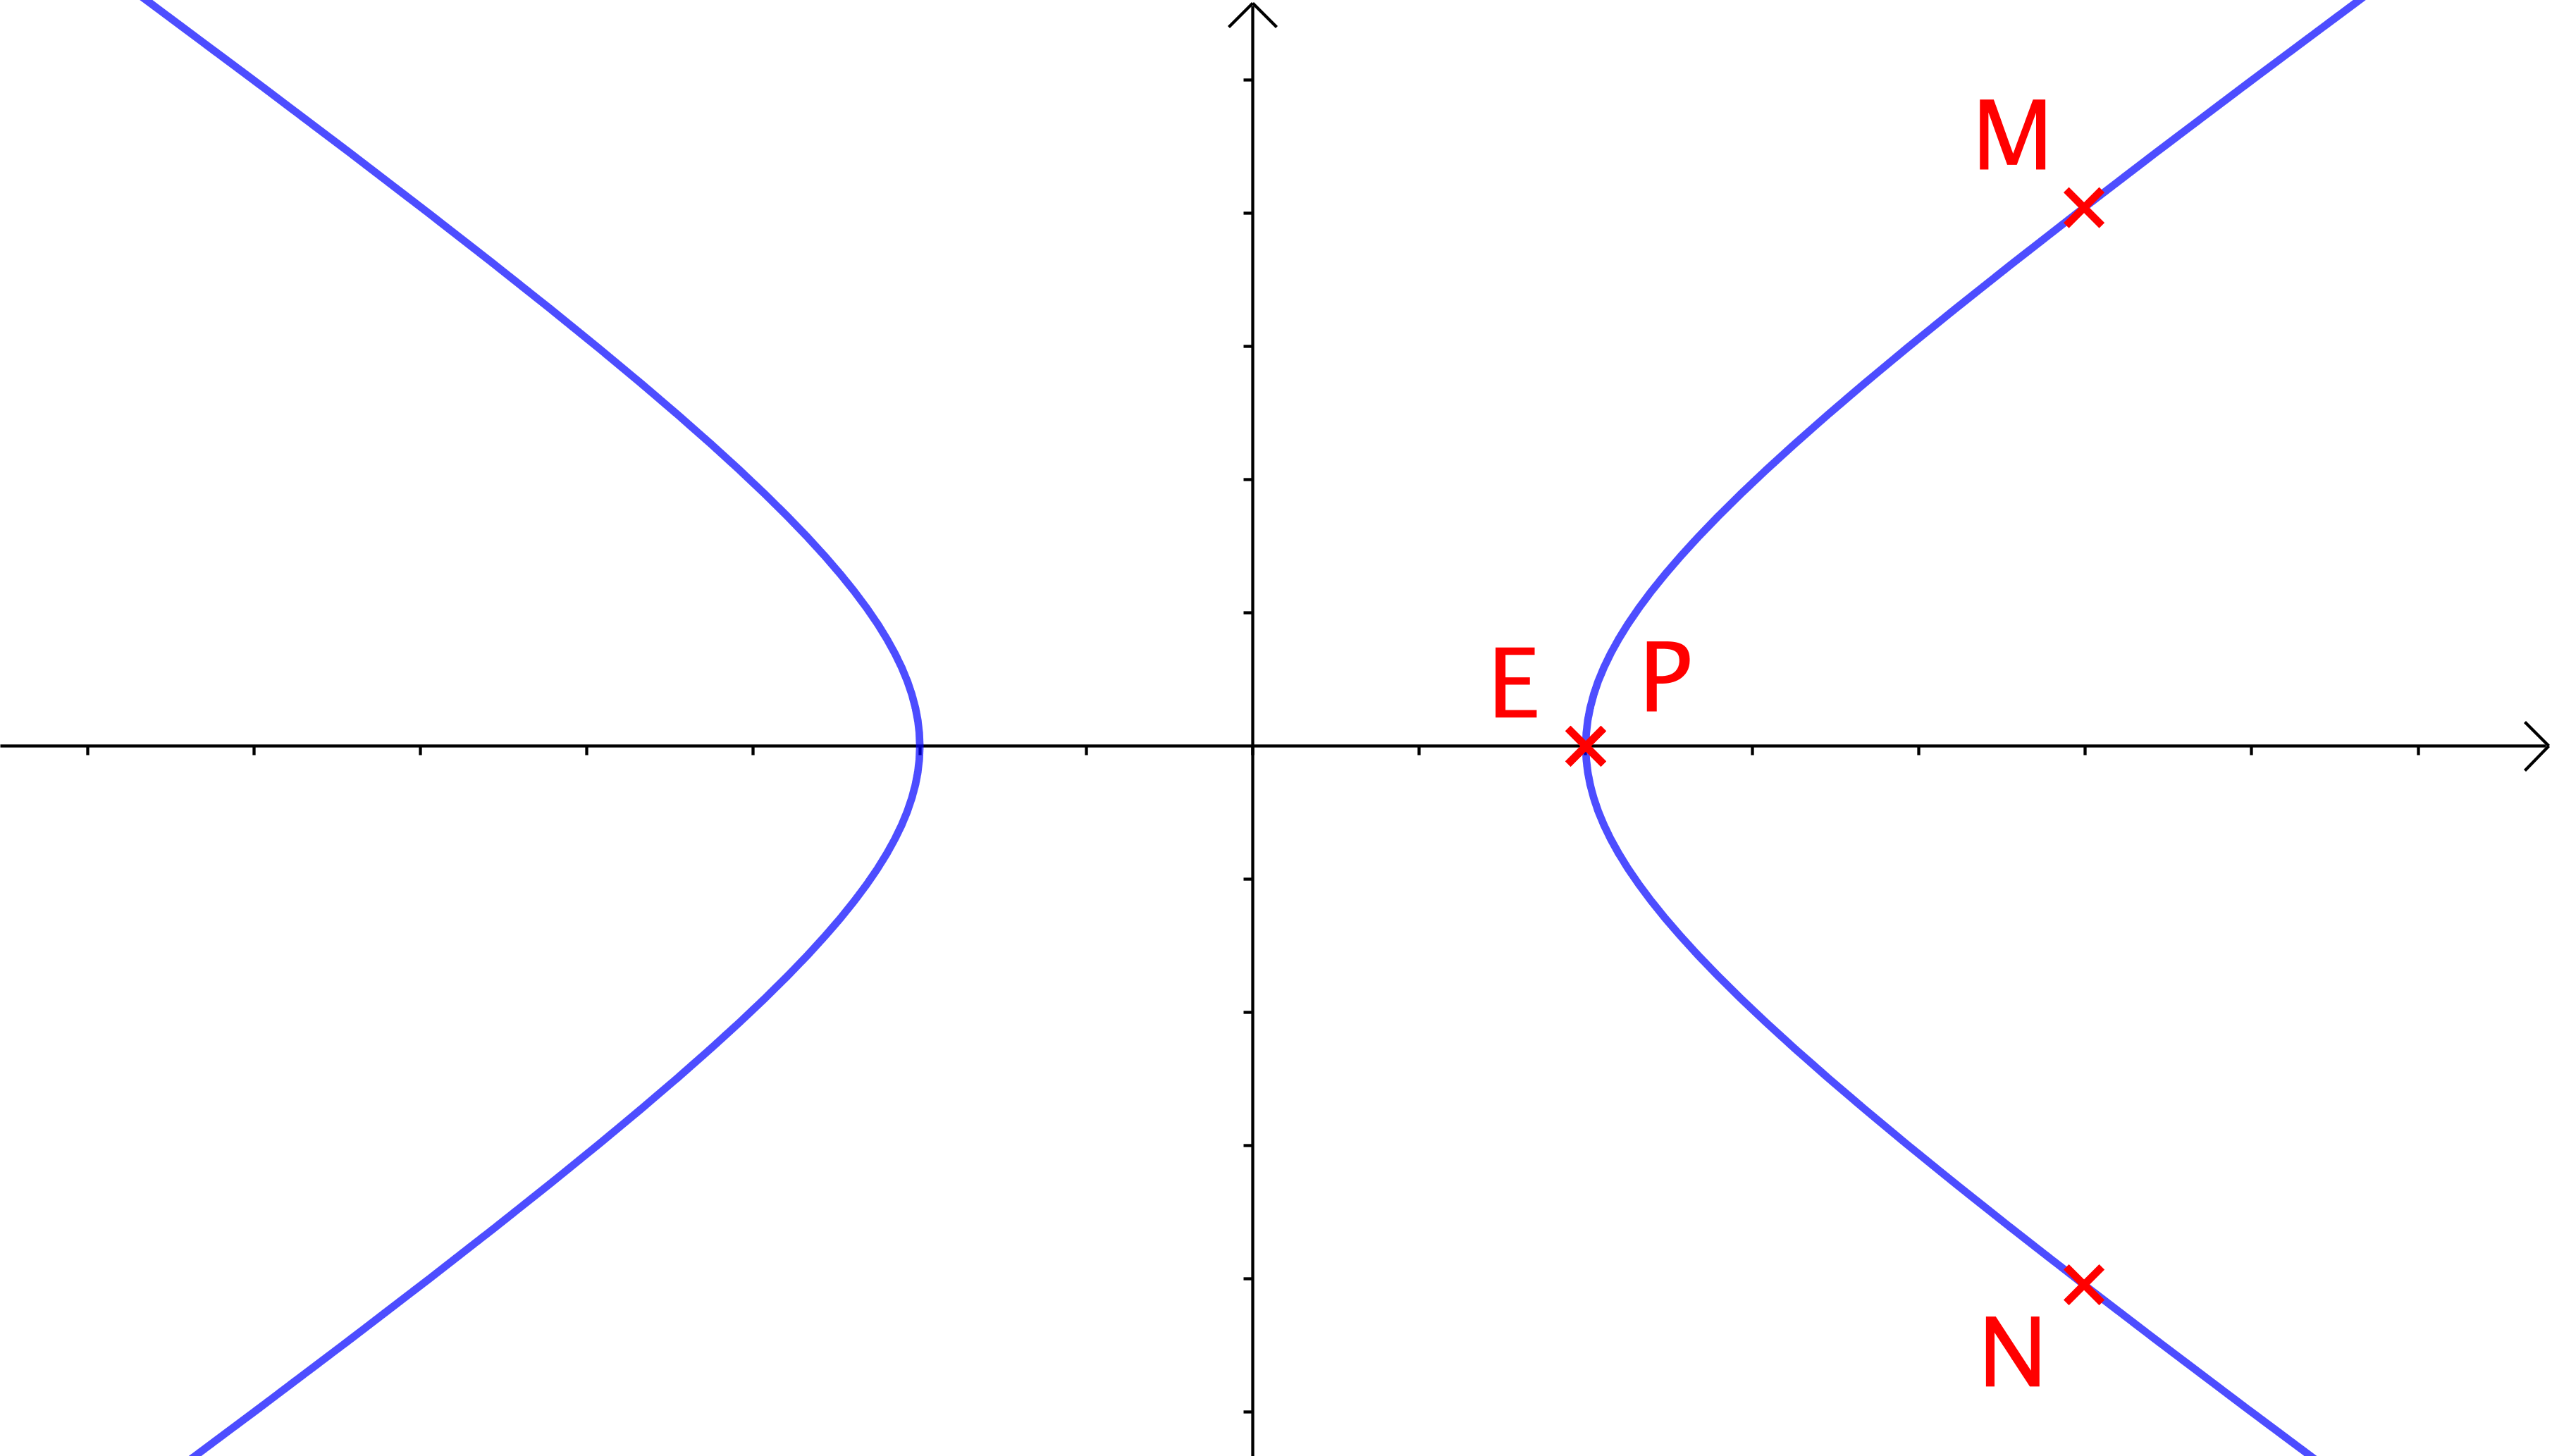
\includegraphics[scale =.5]{exo-spe-math-bac-s-juin-2018/geometry-is-the-queen/vertical-case.png}}

	\columnbreak
	
	\fbox{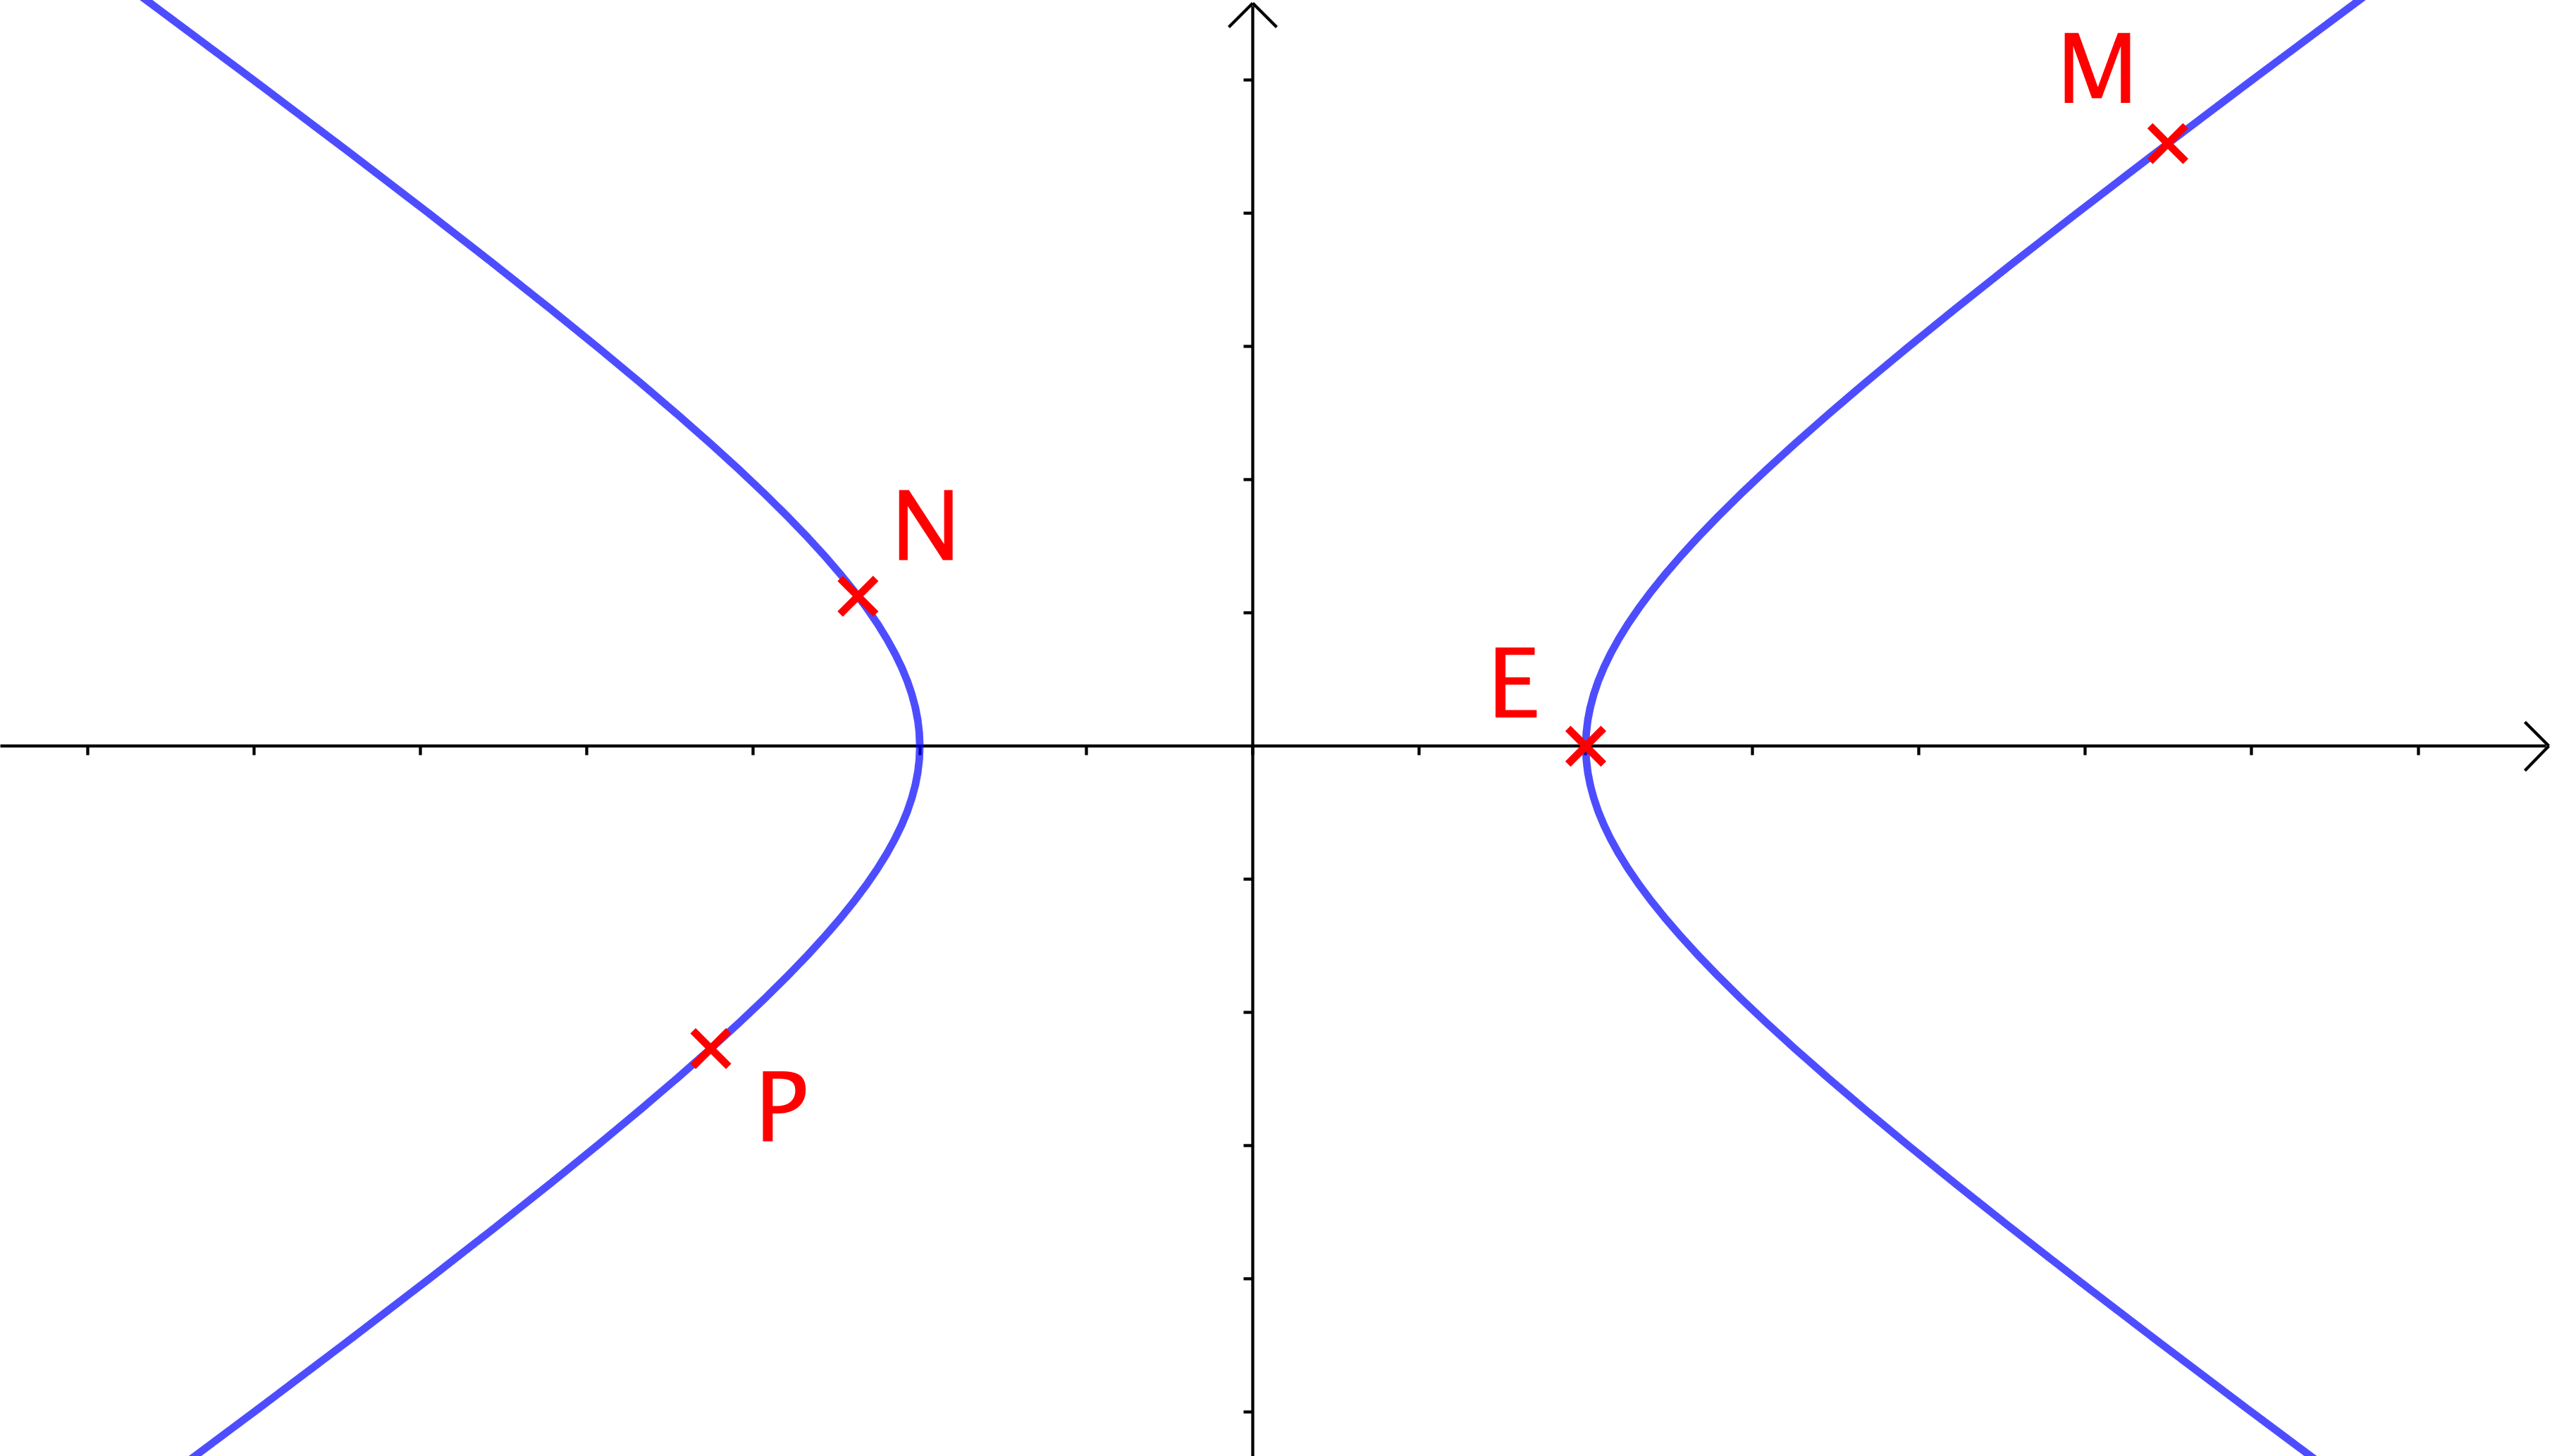
\includegraphics[scale =.5]{exo-spe-math-bac-s-juin-2018/geometry-is-the-queen/oblic-2.png}}
	
	\medskip

	\fbox{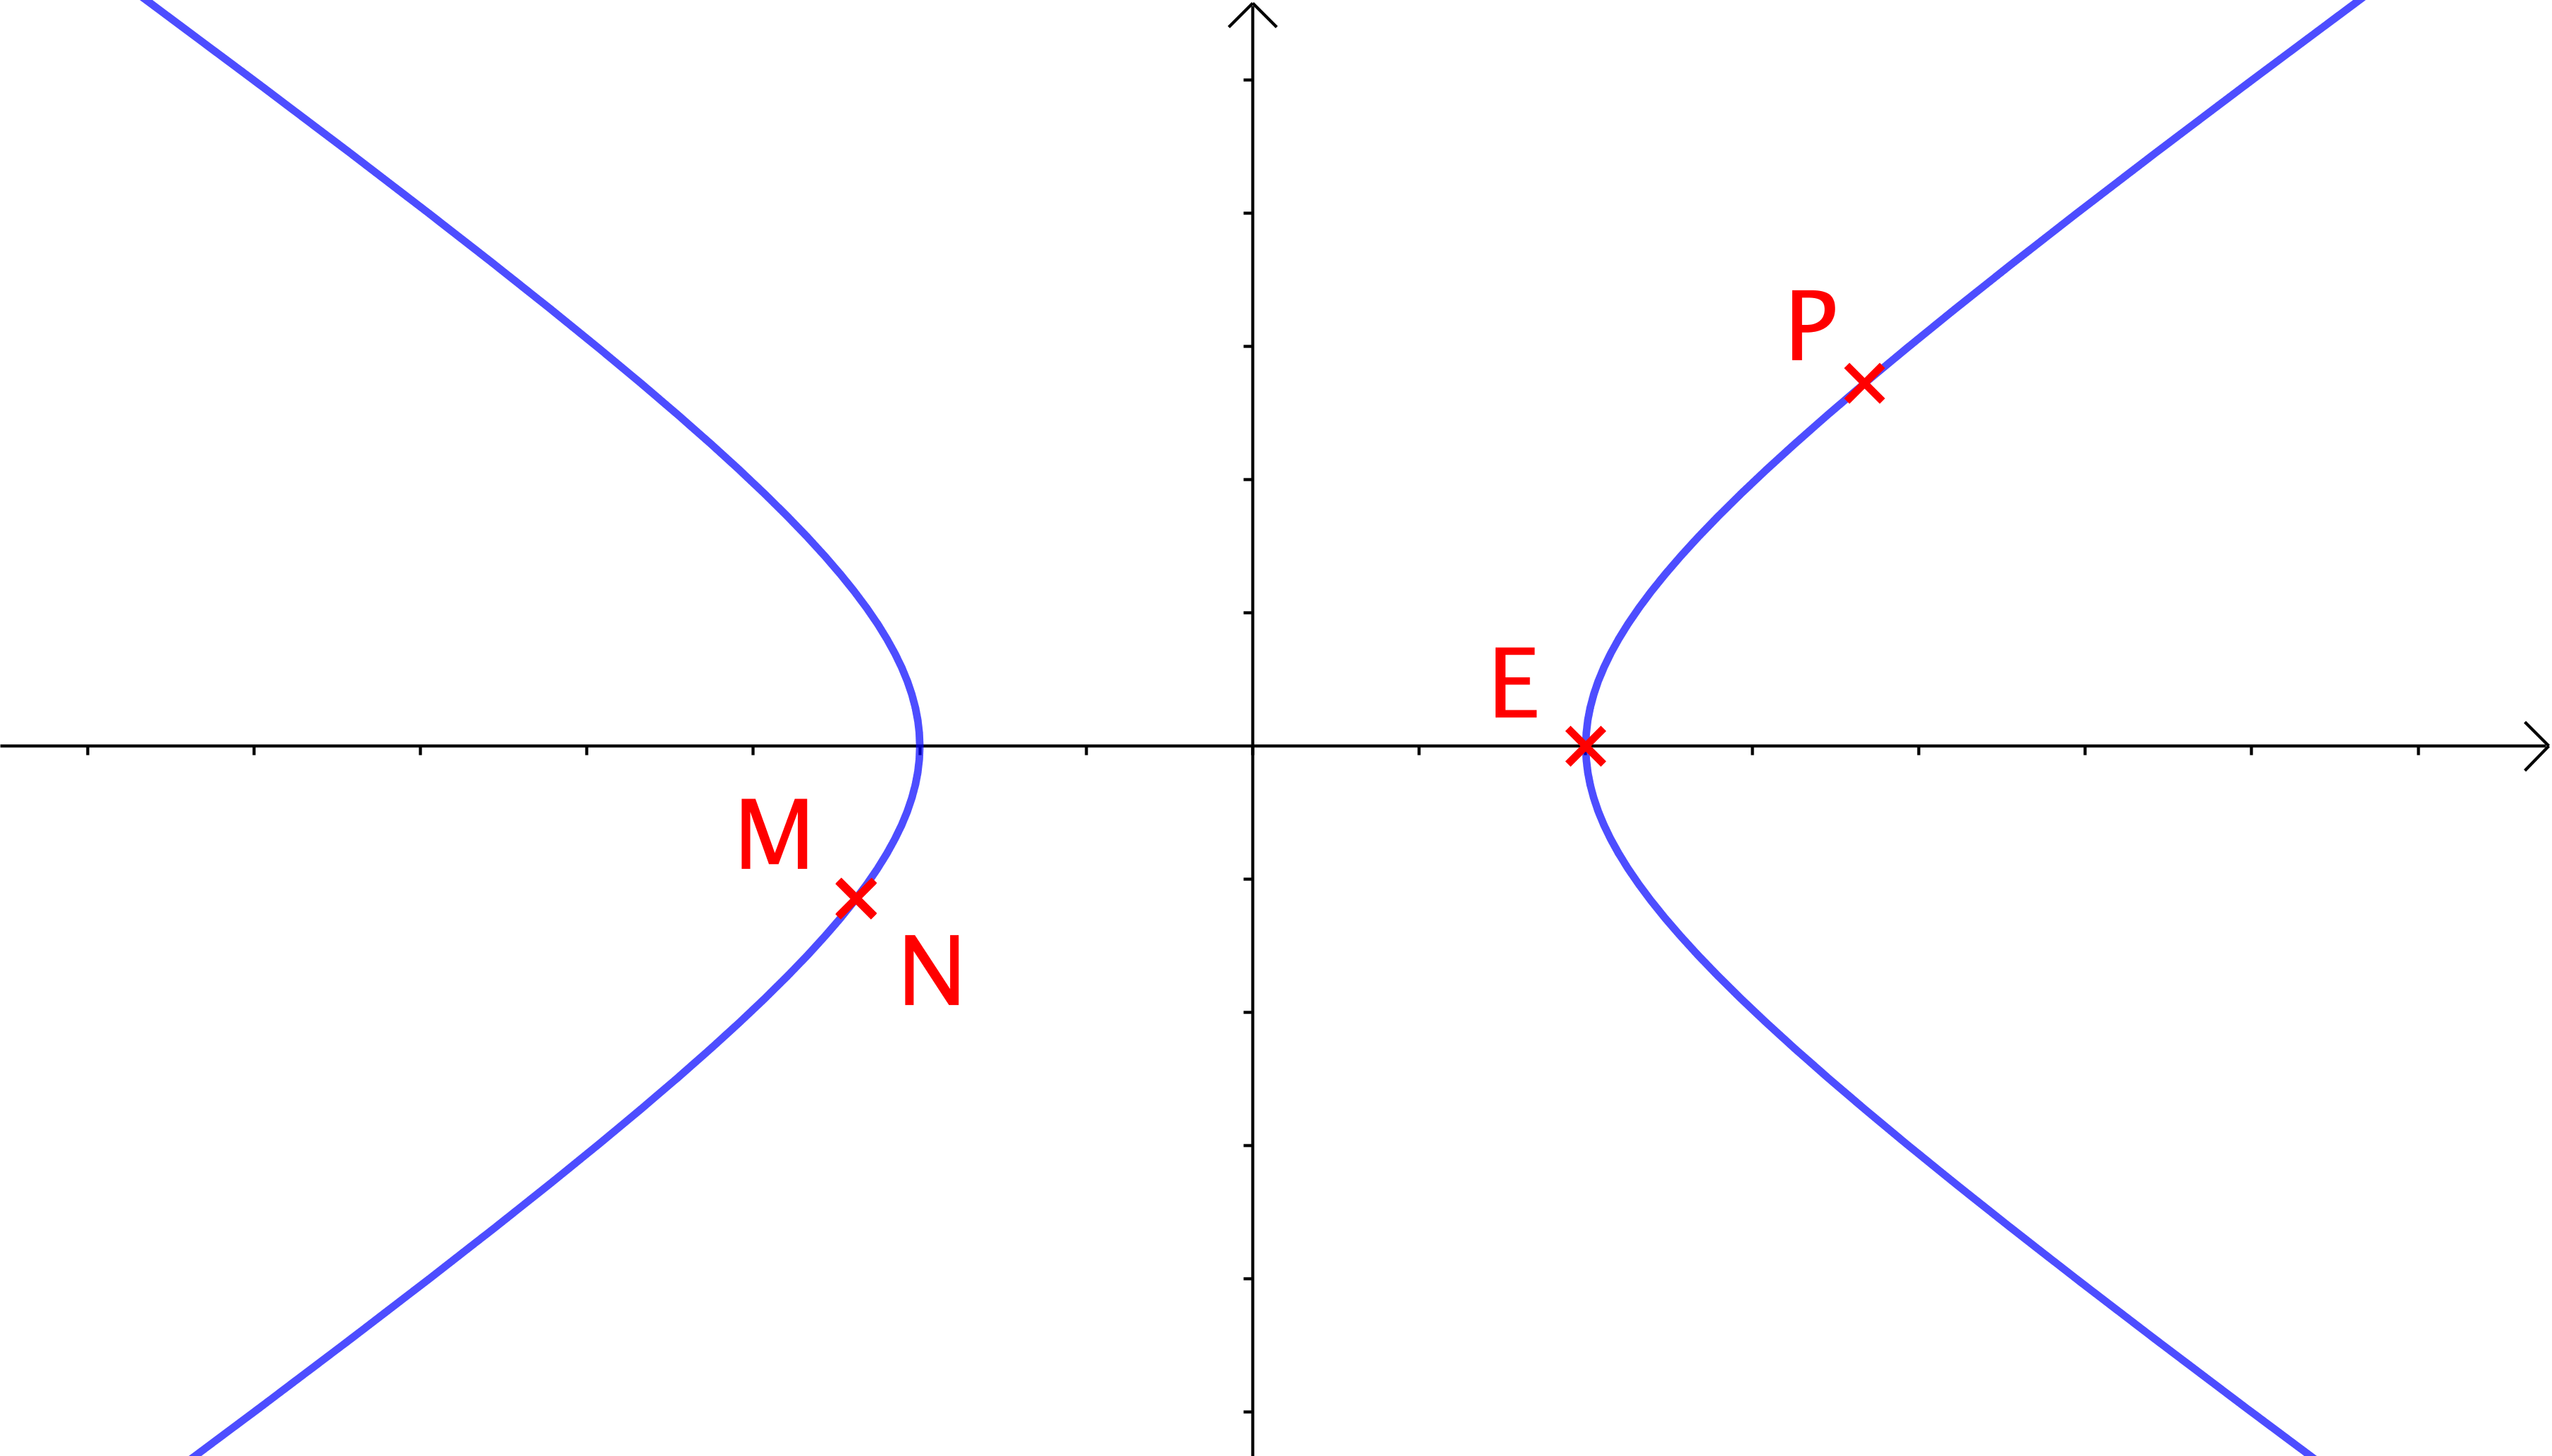
\includegraphics[scale =.5]{exo-spe-math-bac-s-juin-2018/geometry-is-the-queen/same-points.png}}
\end{multicols}


\medskip
	

Les graphiques précédents suggèrent
\footnote{
	Le lieu de téléchargement de ce document contient un fichier GeoGebra \texttt{base-tool.ggb} manipulable dynamiquement pour vérifier combien il est aisé de conjecturer la construction géométrique.
}
un procédé géométrique simple pour construire $P$.

\begin{enumerate}
	\item Si $M \neq N$ et $x \neq x'$, alors $P$ est le second point d'intersection de $\setgeo{H}$ avec la parallèle à $(MN)$ passant par $E$.


	\item Si $M \neq N$ et $x = x'$, alors $P = E$ (ce second cas peut être vu comme un cas limite du précédent avec un point d'intersection \squote{double}).


	\item Si $M = N$ et $y \neq 0$, alors $P$ est le second point d'intersection de $\setgeo{H}$ avec la parallèle de la tangente à $\setgeo{H}$ au point $M$.


	\item Si $M = N$ et $y = 0$, alors $P = E$
	(ce dernier cas peut être vu comme un cas limite du précédent avec un point d'intersection \squote{double}).

\end{enumerate}


Dans les graphiques suivants, nous avons tracé les droites indiquées par le procédé géométrique conjecturé à l'instant.


\medskip


\begin{multicols}{2}
	\center
	
	\fbox{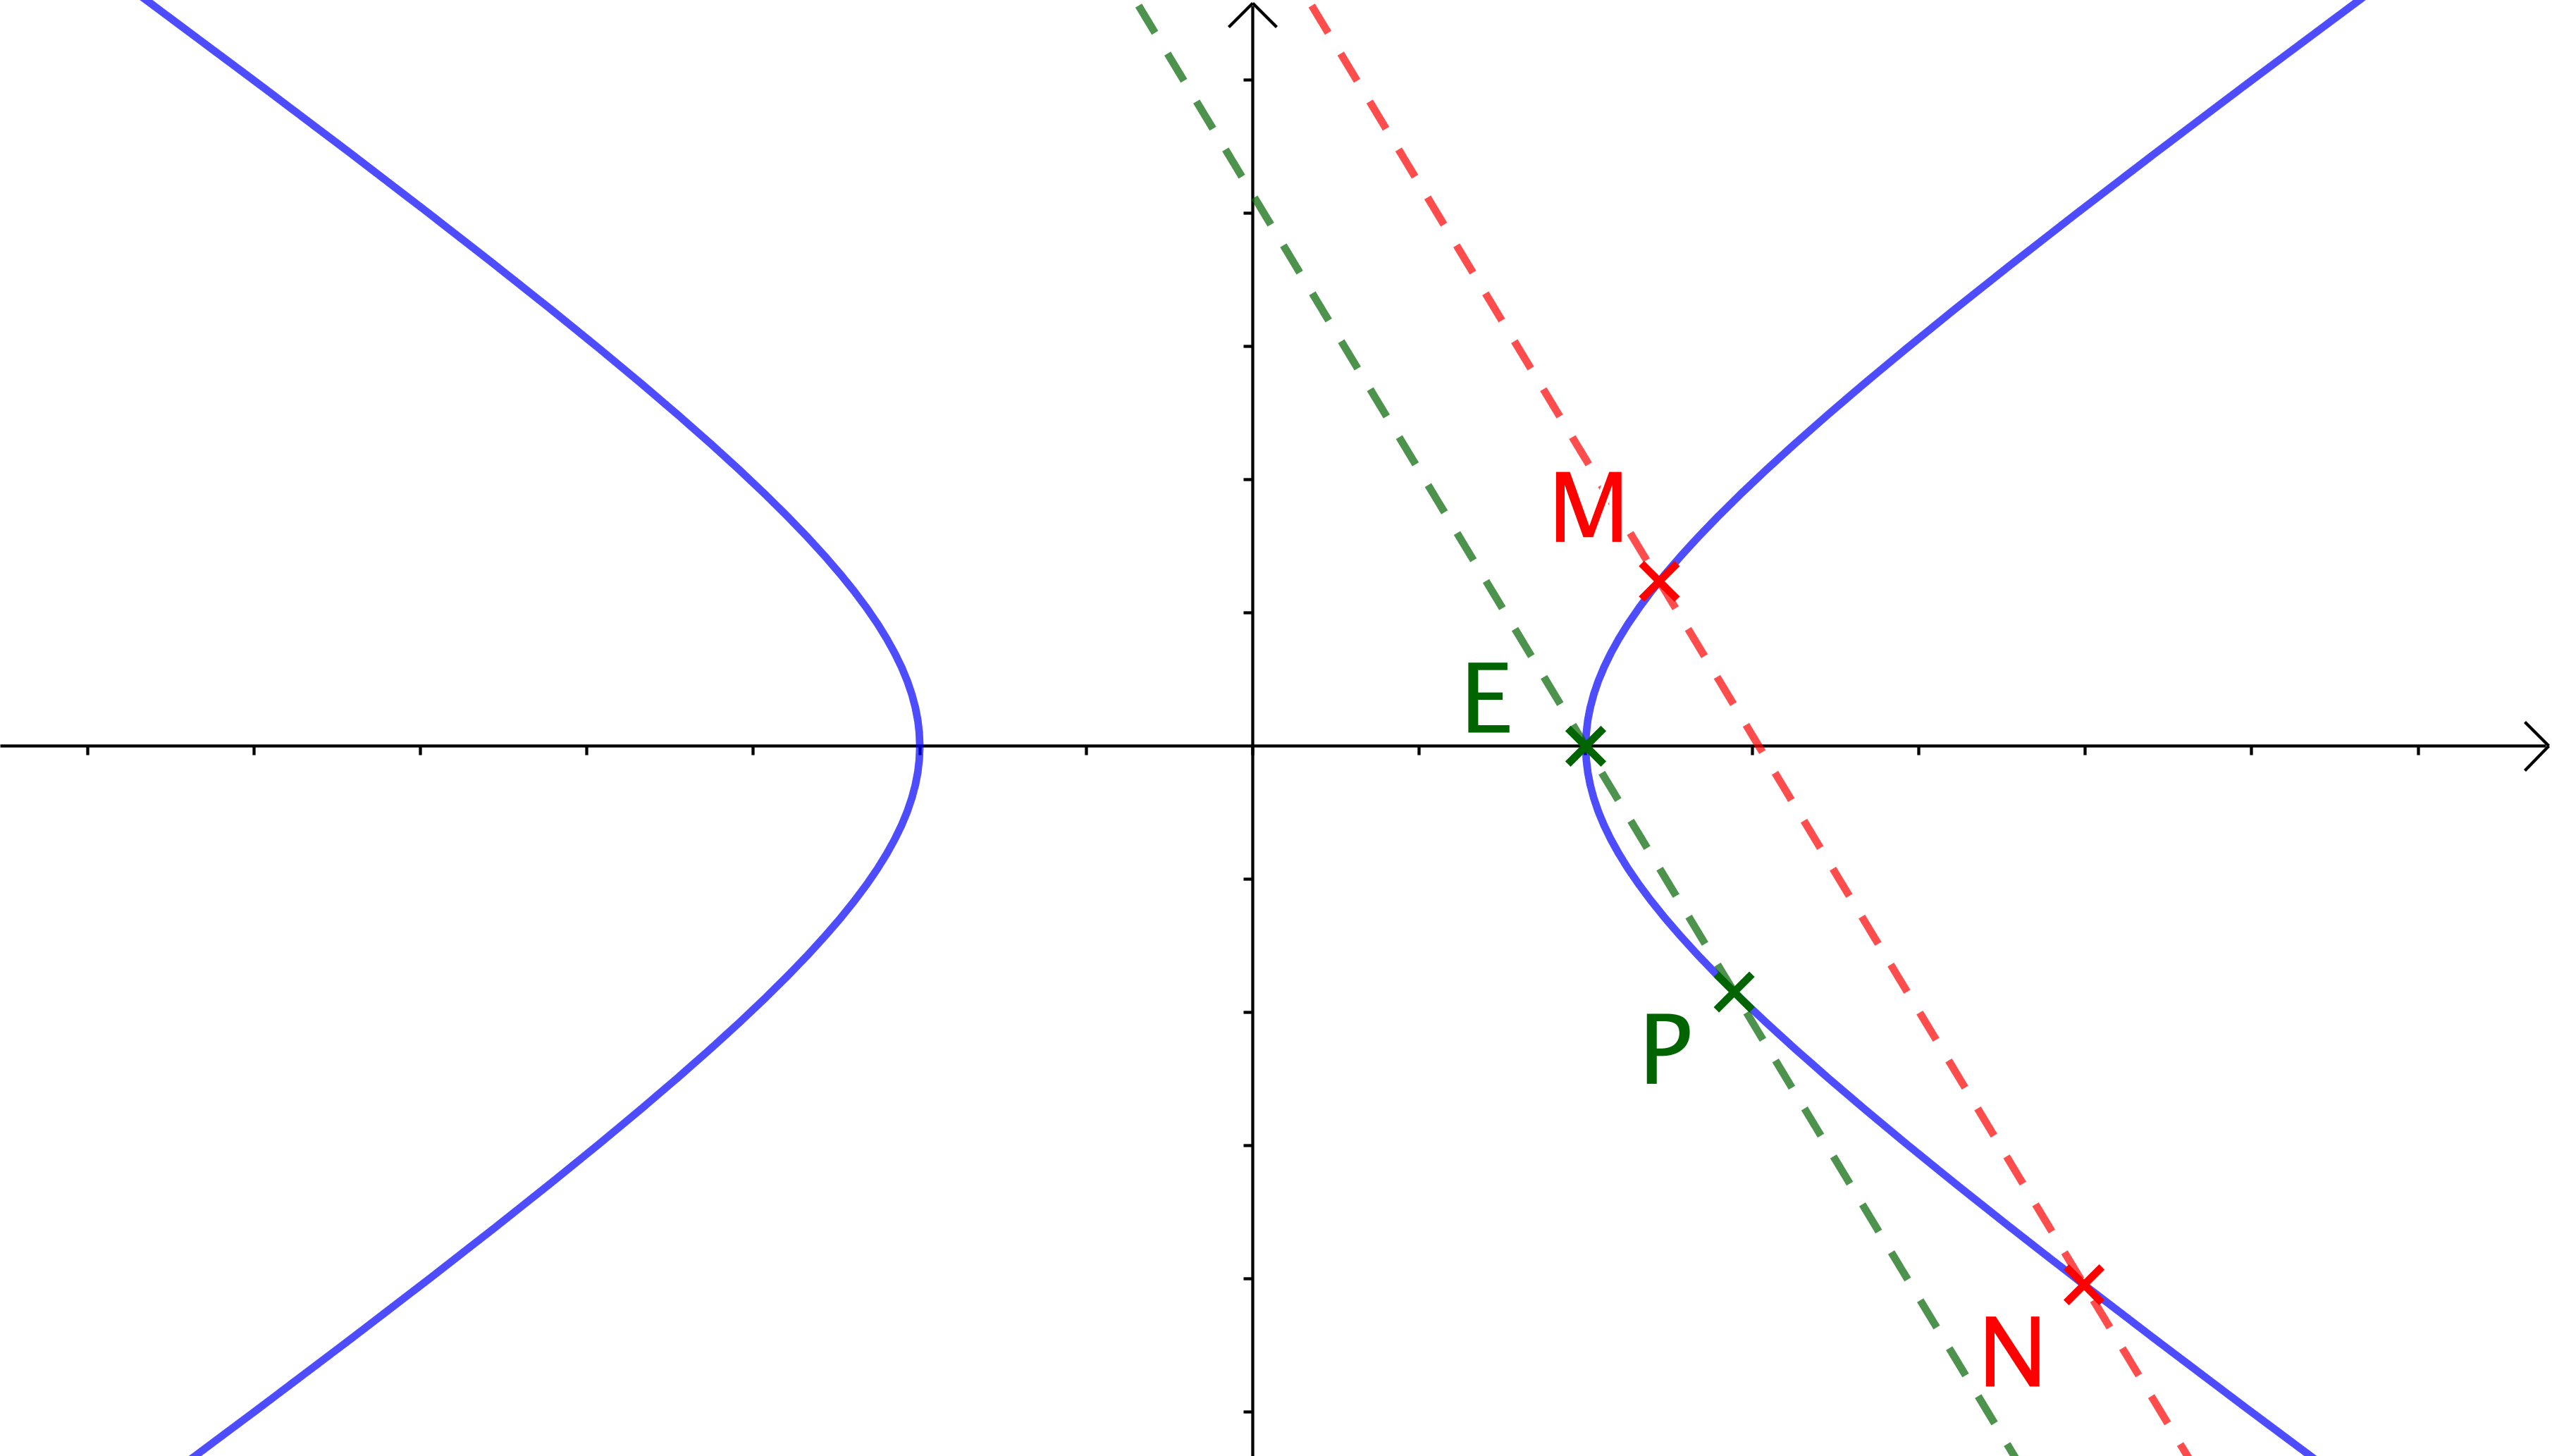
\includegraphics[scale =.5]{exo-spe-math-bac-s-juin-2018/geometry-is-the-queen/oblic-1-with-lines.png}}
	
	\medskip
	
	\fbox{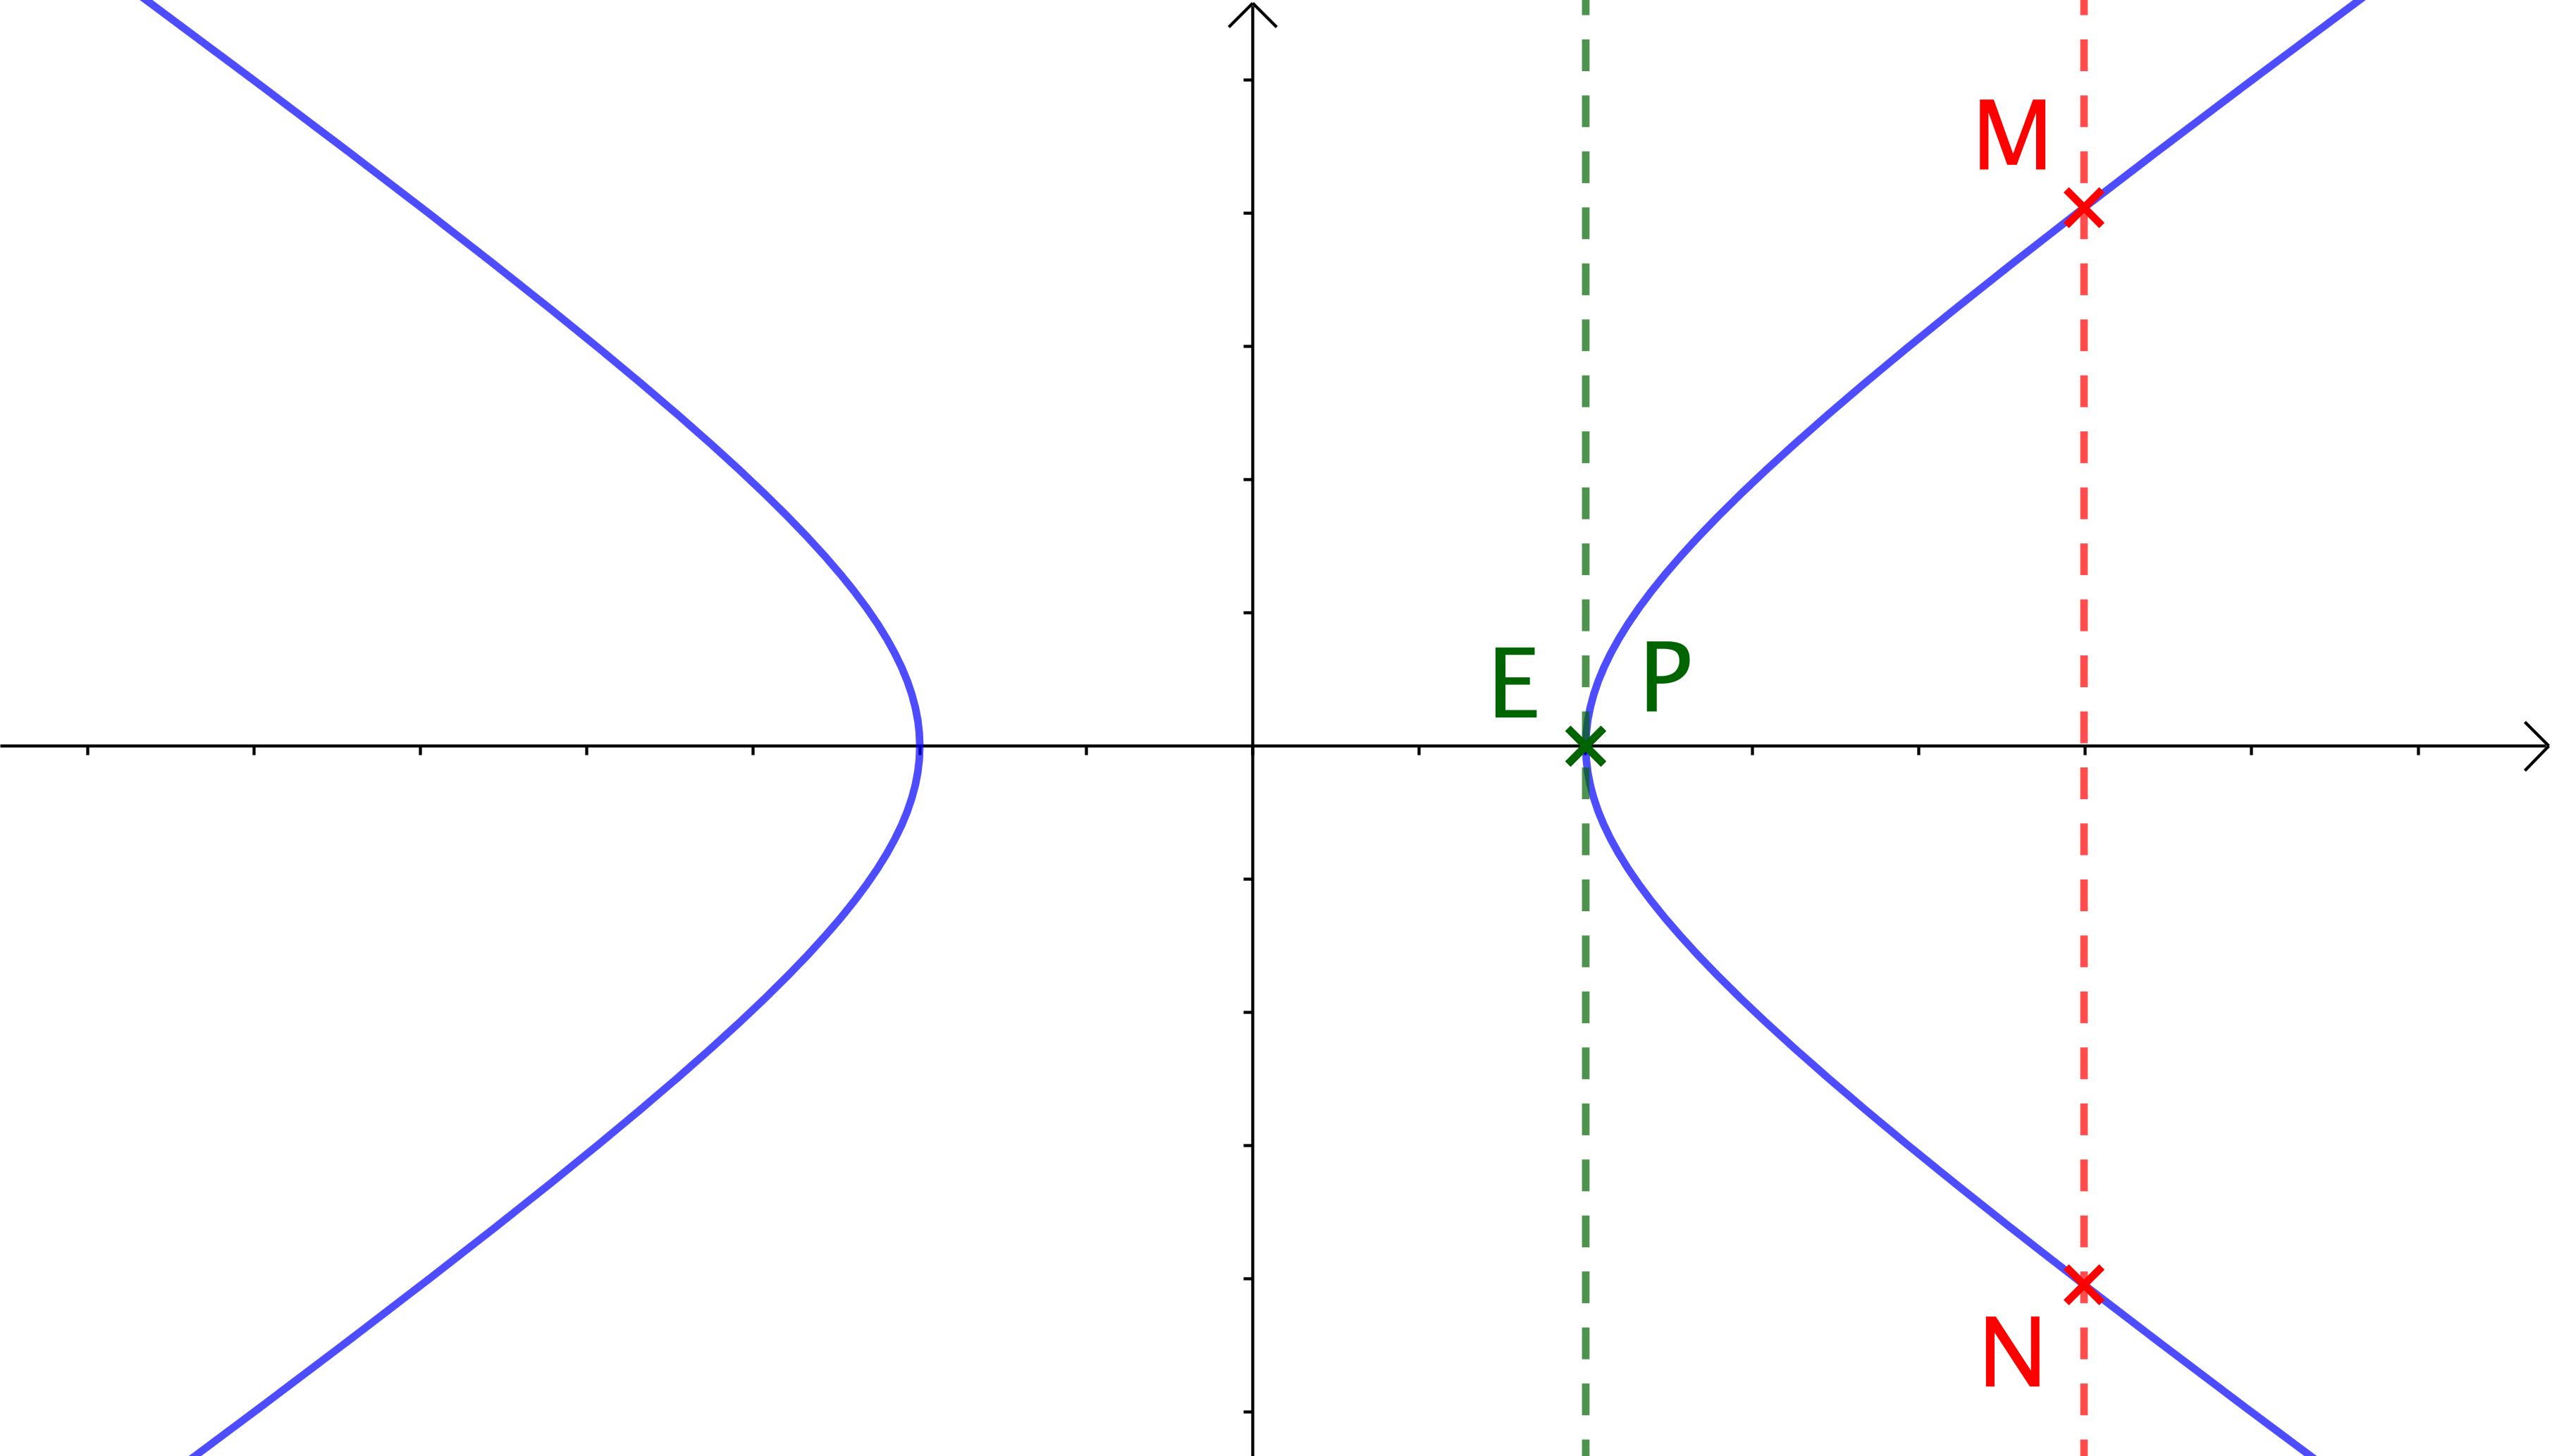
\includegraphics[scale =.5]{exo-spe-math-bac-s-juin-2018/geometry-is-the-queen/vertical-case-with-lines.png}}

	\columnbreak
	
	\fbox{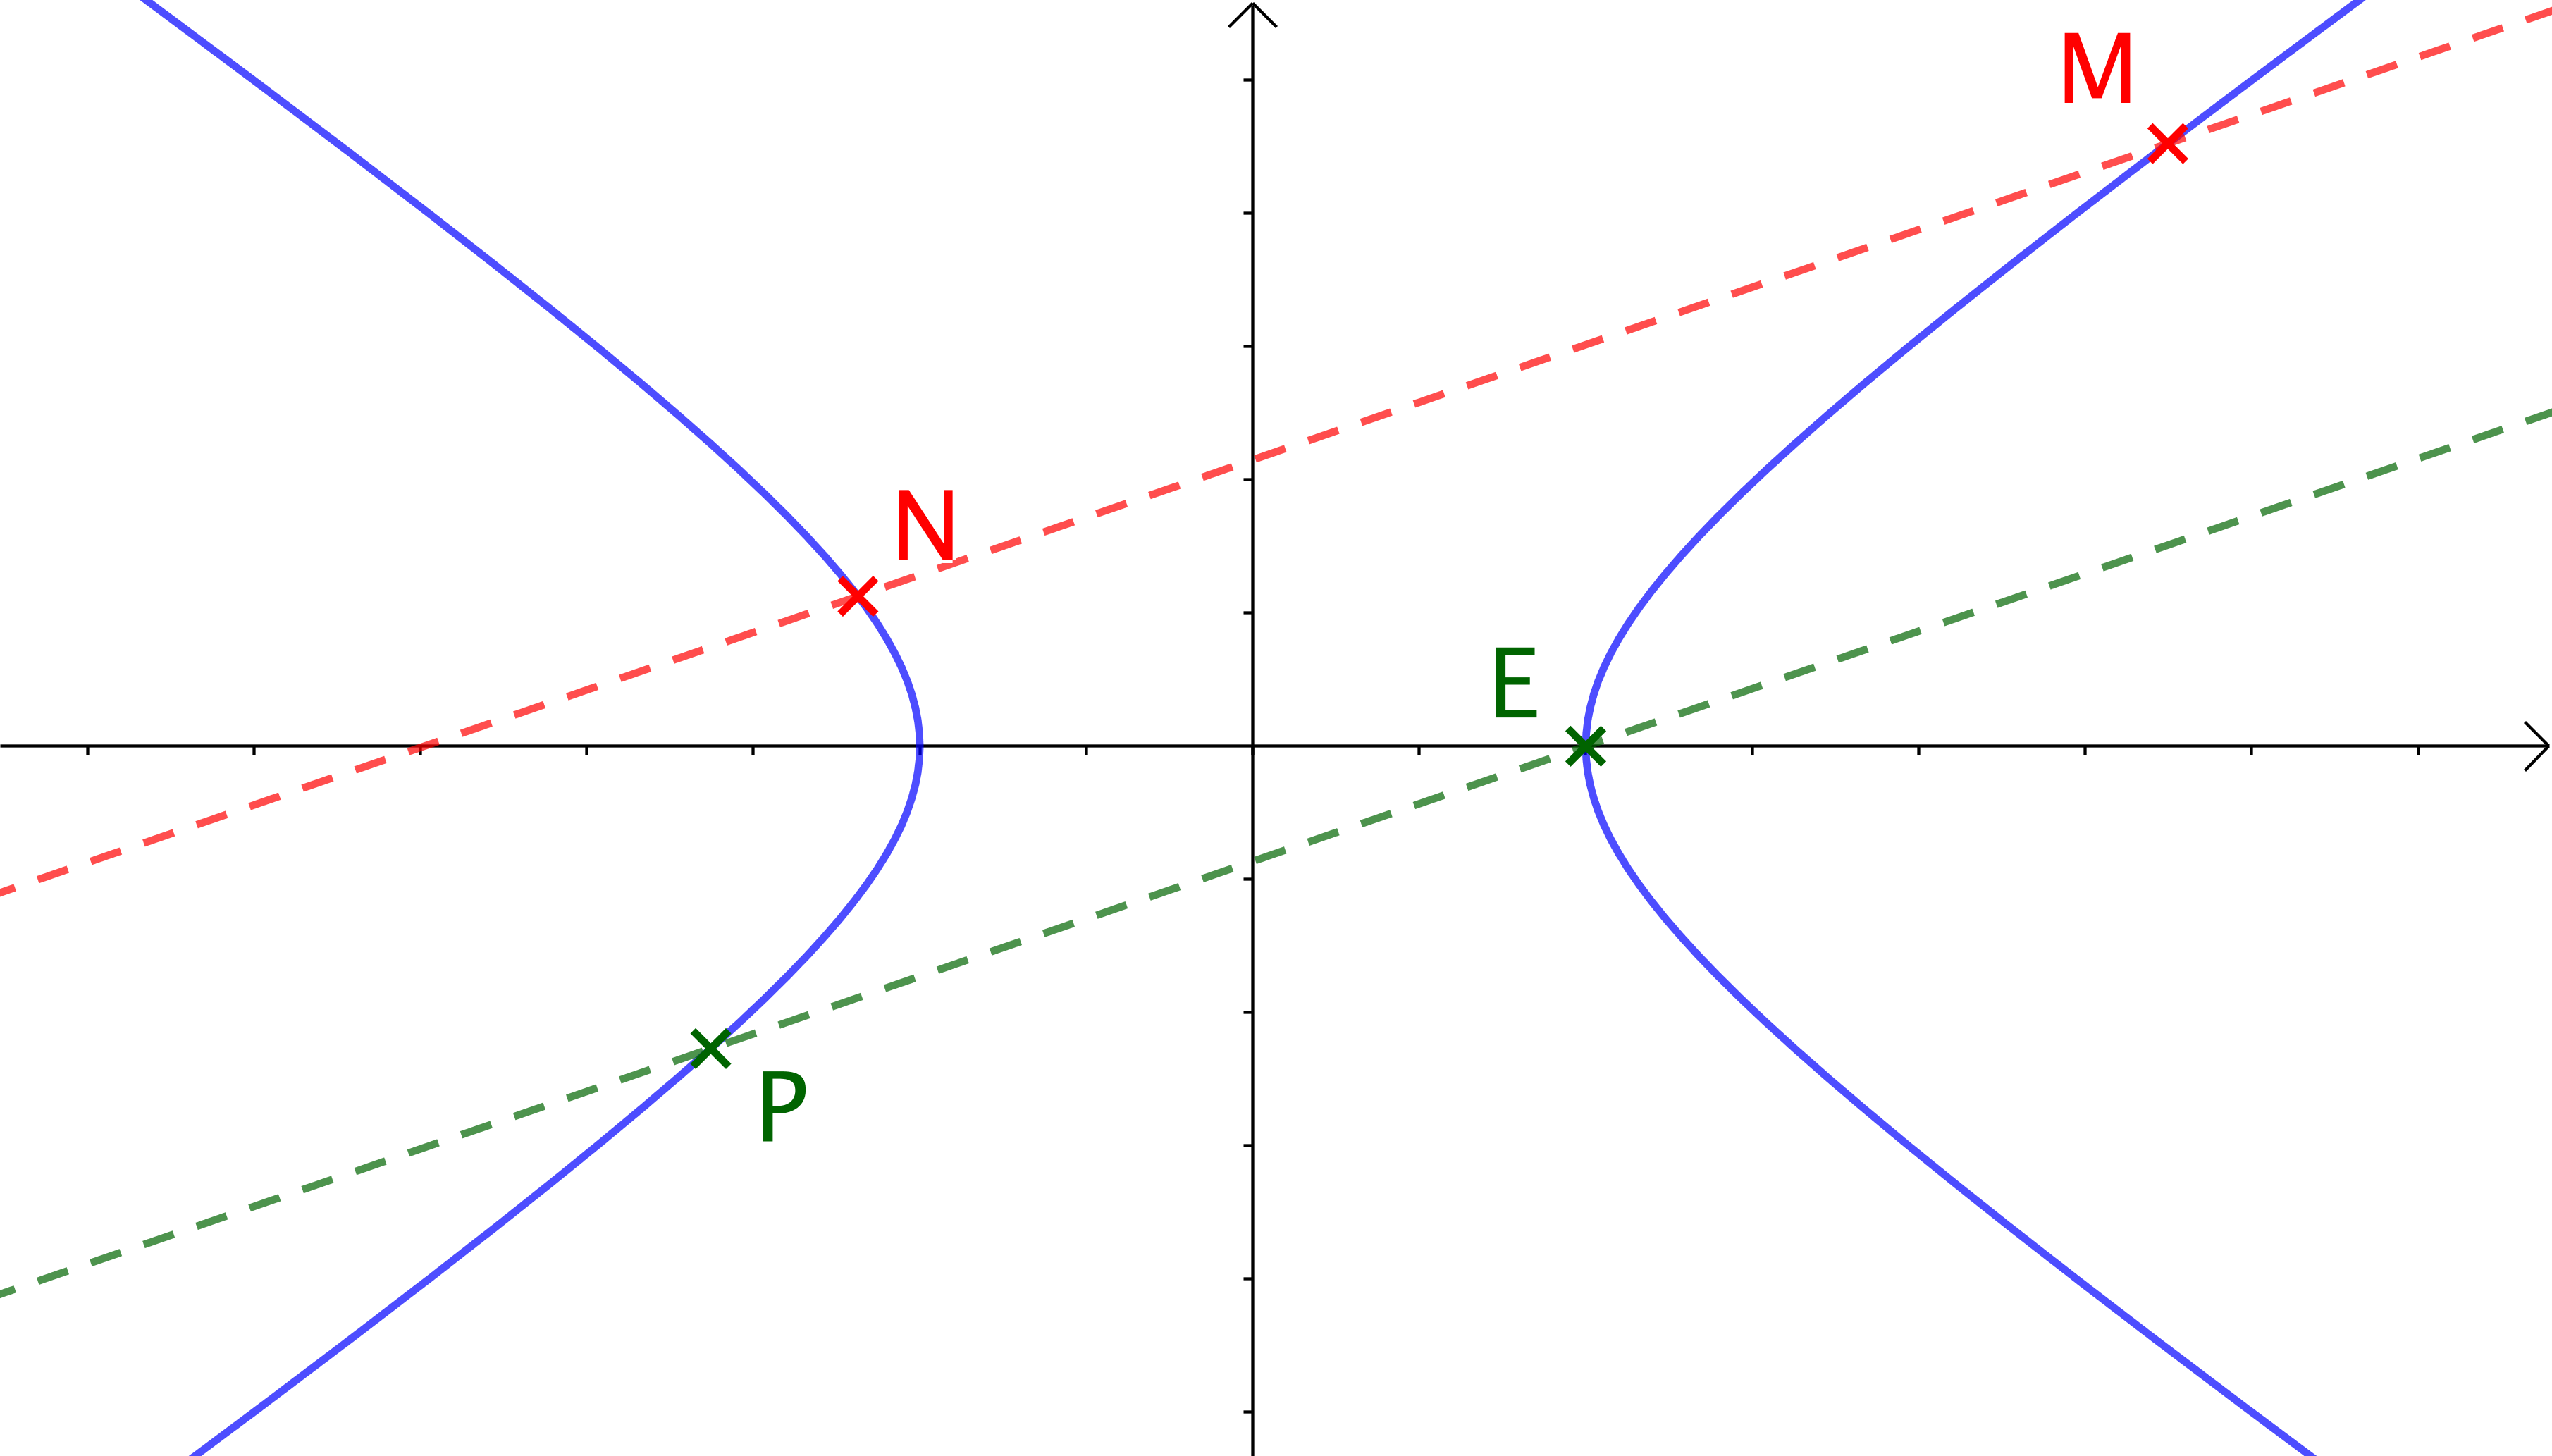
\includegraphics[scale =.5]{exo-spe-math-bac-s-juin-2018/geometry-is-the-queen/oblic-2-with-lines.png}}
	
	\medskip

	\fbox{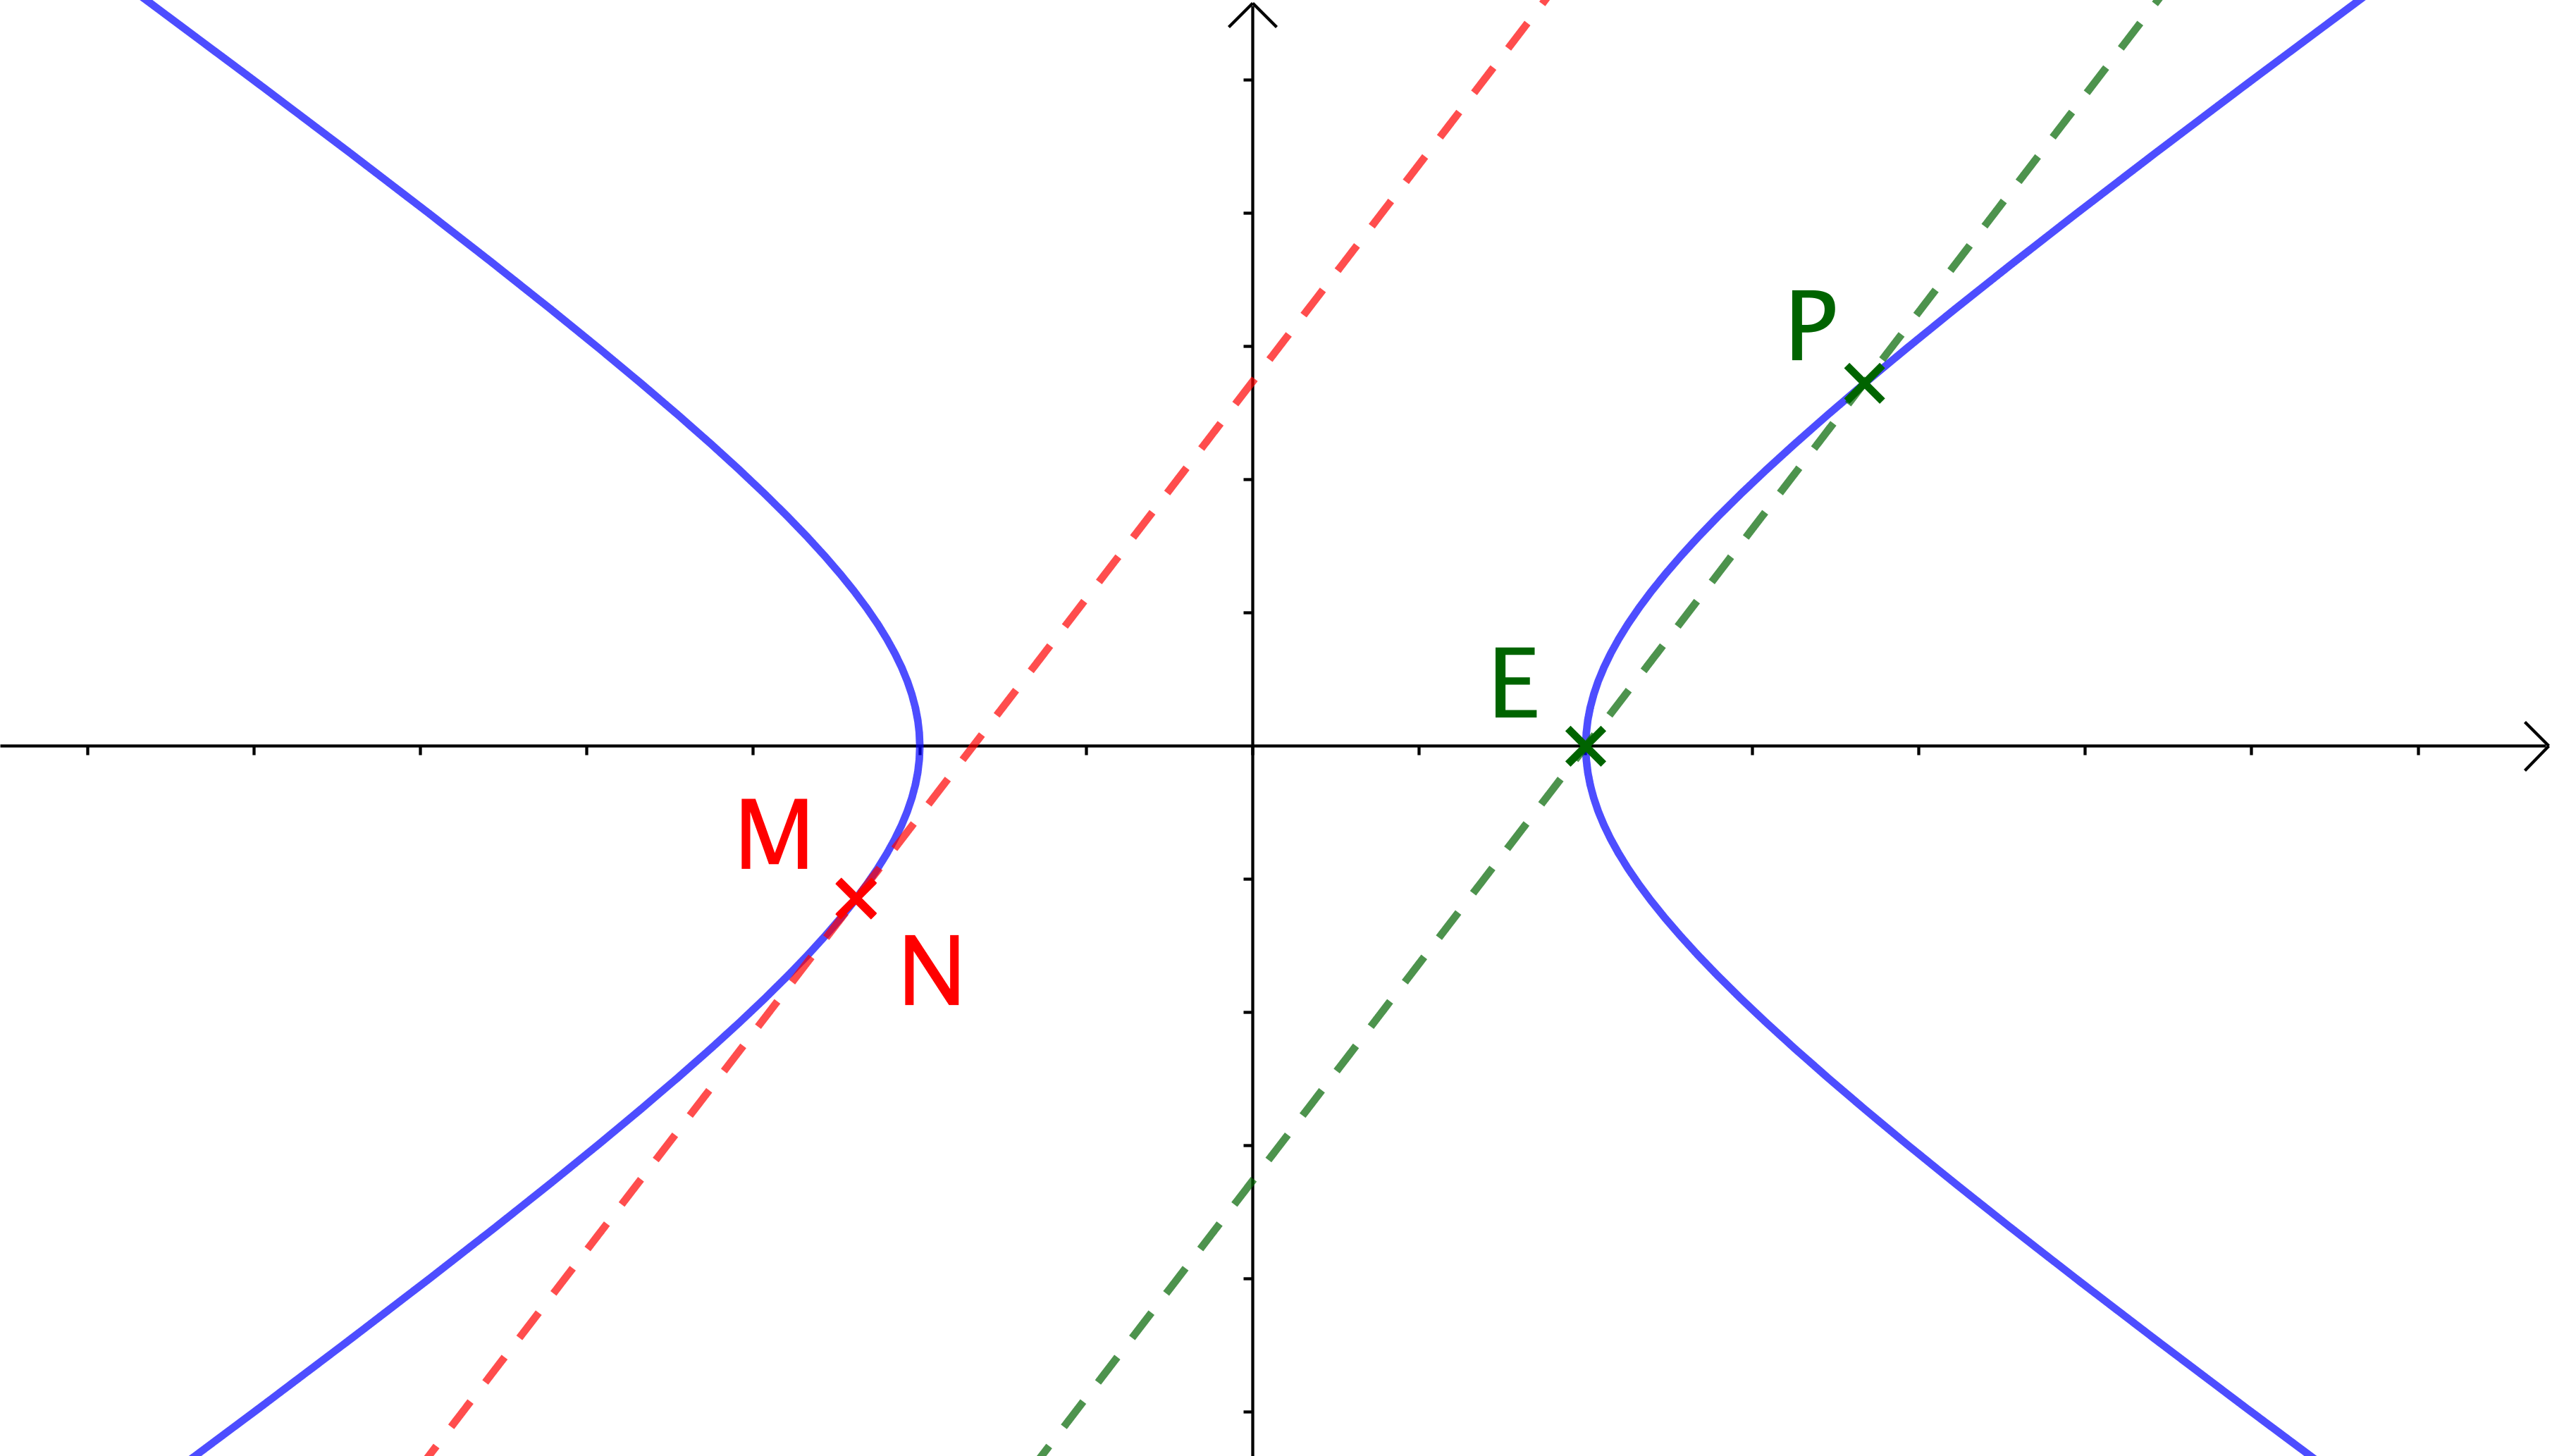
\includegraphics[scale =.5]{exo-spe-math-bac-s-juin-2018/geometry-is-the-queen/same-points-with-lines.png}}
\end{multicols}


\medskip


Comme $E(1 ; 0)$ correspond au neutre de $\star$, il est immédiat que les procédés de construction sont vrais lorsque $M = E$ ou $N = E$.
Prouvons donc la validité de notre conjecture pour $M \neq E$ et $N \neq E$. %Nous confondrons les points avec les vecteurs utilisés pour définir la loi $\star$.

\begin{enumerate}
	\item Supposons $M \neq N$ et $x \neq x'$.
	
	\smallskip
	
	\noindent
	Nous devons vérifier que $P \neq E$, puis le parallélisme de $(EP)$ et $(MN)$.
	
	\smallskip
		
	\noindent
	Démontrons par l'absurde que $P \neq E$. Partons donc de $(x'' ; y'') = (1 ; 0)$,
	c'est-à-dire de $x x' + 8 y y' = 1$ et $x y' + x' y = 0$.
	Nous avons alors:
	
	\medskip
	
	\noindent
	\kern-1em\begin{stepcalc}[style = ar*, ope = {\implies[donc]}]
	    (x x' + 8 y y')^2 = 1
	\explnext{}
	    x^2 x'^2 + 64 y^2 y'^2 + 16 x x' y y' = 1
	\explnext*{$x' y = - x y'$}{}
	    x^2 x'^2 + 64 y^2 y'^2 - 16 x^2 y'^2 = 1
	\explnext*{$x^2 = 1 + 8 y^2$ et $x'^2 = 1 + 8 y'^2$}{}
	      (1 + 8 y^2) (1 + 8 y'^2) 
	    + 64 y^2 y'^2 
	    - 16 (1 + 8 y^2) y'^2 
	    = 1
	\explnext{}
	      1 + 8 y^2 + 8 y'^2 + 64 y^2 y'^2 
	    + 64 y^2 y'^2 
	    - 16 y'^2 - 128 y^2 y'^2
	    = 1
	\explnext{}
	    8 y^2 - 8 y'^2 = 0
	\explnext{}
	    y^2 = y'^2
	\explnext{}
	    y = \pm y'
	\end{stepcalc}
	
	\medskip
		
	\noindent
	Or $y = y'= 0$ est exclus ici, puisque $M \neq E$ et $N \neq E$.
	Donc,
	$y = \pm y'$ donne $y \neq 0$ et $y'\neq 0$, puis $x' y = - x y'$ et $x \neq x'$ impliquent
	$(x' ; y') = (- x ; y)$.
	Nous obtenons alors
	$x x' + 8 y y' = - x^2 + 8 y^2 = -1$ qui contredit $x x' + 8 y y' = 1$.
	
	\smallskip
		
	\noindent
	Ensuite, le parallélisme des droites $(EP)$ et $(MN)$ se démontrent via les calculs quelque peu brutaux suivants.%
	\footnote{
	    Faire appel à un logiciel de calcul formel serait ici acceptable.
	}
	
	\smallskip
	
	\noindent
	$\det\left ( \vect{EP} ; \vect{MN} \right)
	=
	\left|\begin{NiceArray}{cc} 
	  x'' - 1 & x' - x \\ 
	  y''     & y' - y
	\end{NiceArray}\right|$
	
	\noindent
	$\phantom{\det\left ( \vect{EP} ; \vect{MN} \right)}
	=
	(x'' - 1)(y' - y) -  y'' (x' - x)$
	
	\noindent
	$\phantom{\det\left ( \vect{EP} ; \vect{MN} \right)}
	=
	(x x' + 8 y y' - 1)(y' - y) -  (y x' + x y') (x' - x)$
	
	\noindent
	$\phantom{\det\left ( \vect{EP} ; \vect{MN} \right)}
	=
	x x' y' + 8 y y'^2 - y' - x x' y - 8 y^2 y' + y
	- 
	y x'^2 - x x' y' + y x x' + x^2 y'$
	
	\noindent
	$\phantom{\det\left ( \vect{EP} ; \vect{MN} \right)}
	=
	8 y y'^2 - y' - 8 y^2 y' + y
	- 
	y x'^2 + x^2 y'$
	
	\smallskip
	
	\noindent
	Réordonnons les termes en nous souvenant que $x^2 - 8 y^2 = 1$ et $x'^2 - 8 y'^2 = 1$.

	\smallskip
	
	\noindent
	${\det\left ( \vect{EP} ; \vect{MN} \right)}
	=
	x^2 y' - 8 y^2 y'
	- y x'^2 + 8 y y'^2
	- y' + y$
	
	\noindent
	$\phantom{\det\left ( \vect{EP} ; \vect{MN} \right)}
	=
	(x^2 - 8 y^2)y'
	- y(x'^2 - 8 y'^2)
	- y' + y$
	
	\noindent
	$\phantom{\det\left ( \vect{EP} ; \vect{MN} \right)}
	=
	y'
	- y
	- y' + y$
	
	\noindent
	$\phantom{\det\left ( \vect{EP} ; \vect{MN} \right)}
	=
	0$
	
	\smallskip
	
	\noindent
	Les vecteurs $\vect{EP}$ et $\vect{MN}$ sont bien colinéaires.

% --------------- %

	\medskip
	\item Supposons $M \neq N$ et $x = x'$.
	
	\smallskip
	
	\noindent
	Dans ce cas, 
	nous avons aussi $y' = - y$, 
	d'où
	$x'' = x x' + 8 y y' = x^2 - 8 y^2 = 1$
	et
	$y'' = y x' + x y' = y x - x y = 0$.
	Ceci justifie que $P = E$.

% --------------- %

	\medskip
	\item Supposons $M = N$.
	
	\smallskip
	
	\noindent
	$\mathcal{H}: F(X ; Y) = 0$, où $F(X ; Y) = X^2 - 8 Y^2 - 1$,
	admet une tangente en $M$ de vecteur directeur
	$\vect{u} \big( - \pder{F}{Y}{1}(x ; y) ; \pder{F}{X}{1}(x ; y) \big)$ si ce vecteur est non nul.
	
	\noindent
	Comme $\vect{u} ( 16y ; 2x )$ et $(x ; y) \neq (0 ; 0)$, car $x^2 - 8 y^2 - 1 = 0$,
	$\mathcal{H}$ admet en $M$ une tangente de vecteur directeur $\vect{u} ( 16y ; 2x )$.
	%
	Comme de plus $x'' = x^2 + 8y^2 = 16y^2 + 1$ et $y'' = 2xy$, nous avons
	$\vect{EP} ( 16y^2 ; 2xy )$,
	soit $\vect{EP} = y \vect{u}$.
	Deux alternatives sont alors possibles.
	%
	\begin{itemize}
	    \item Si $y = 0$, alors $M(-1 ; 0)$ et $P = E$, via $\vect{EP} = \vect{0}$. Ceci valide le dernier point de la conjecture.

	    \item Si $y \neq 0$, alors $P$ est le second point d'intersection de $\setgeo{H}$ avec la parallèle de la tangente à $\setgeo{H}$ au point $M$. Ceci achève la validation complète de la conjecture.
	\end{itemize}
\end{enumerate}


\medskip


\textbf{Remarque.} L'approche géométrique proposée ici s'adapte à d'autres courbes caractéristiques:
\begin{itemize}
    \item au cercle trigonométrique avec $E(1 ; 0)$;
    \item à la parabole d'équation $y = x^2$ avec $E(0 ; 0)$;
    \item à l'hyperbole d'équation $y = \dfrac{1}{x}$ avec $E(1 ; 1)$.
\end{itemize}
Nous laissons au lecteur le soin de découvrir les structures de groupe sous-jacentes à ces constructions.
Plus généralement, toute conique non dégénérée $\setgeo{C} : a X^2 + b Y^2 + c X Y + d = 0$ peut être munie d'une structure de groupe par ce même procédé, en choisissant un point $E$ quelconque de $\setgeo{C}$ comme élément neutre.
